\RequirePackage{luatex85}
\documentclass[tikz]{standalone}
\usepackage{tikz-qtree}
\usetikzlibrary{shadows,trees}
\tikzset{
edge from parent fork down,
level distance=4cm,
every node/.style=
    {top color=white,
    bottom color=blue!25,
    rectangle,rounded corners,
    minimum height=8mm,
    draw=blue!75,
    very thick,
    drop shadow,
    align=center,
    text depth = 0pt
    },
edge from parent/.style=
    {draw=blue!50,
    thick
    }}
\begin{document}
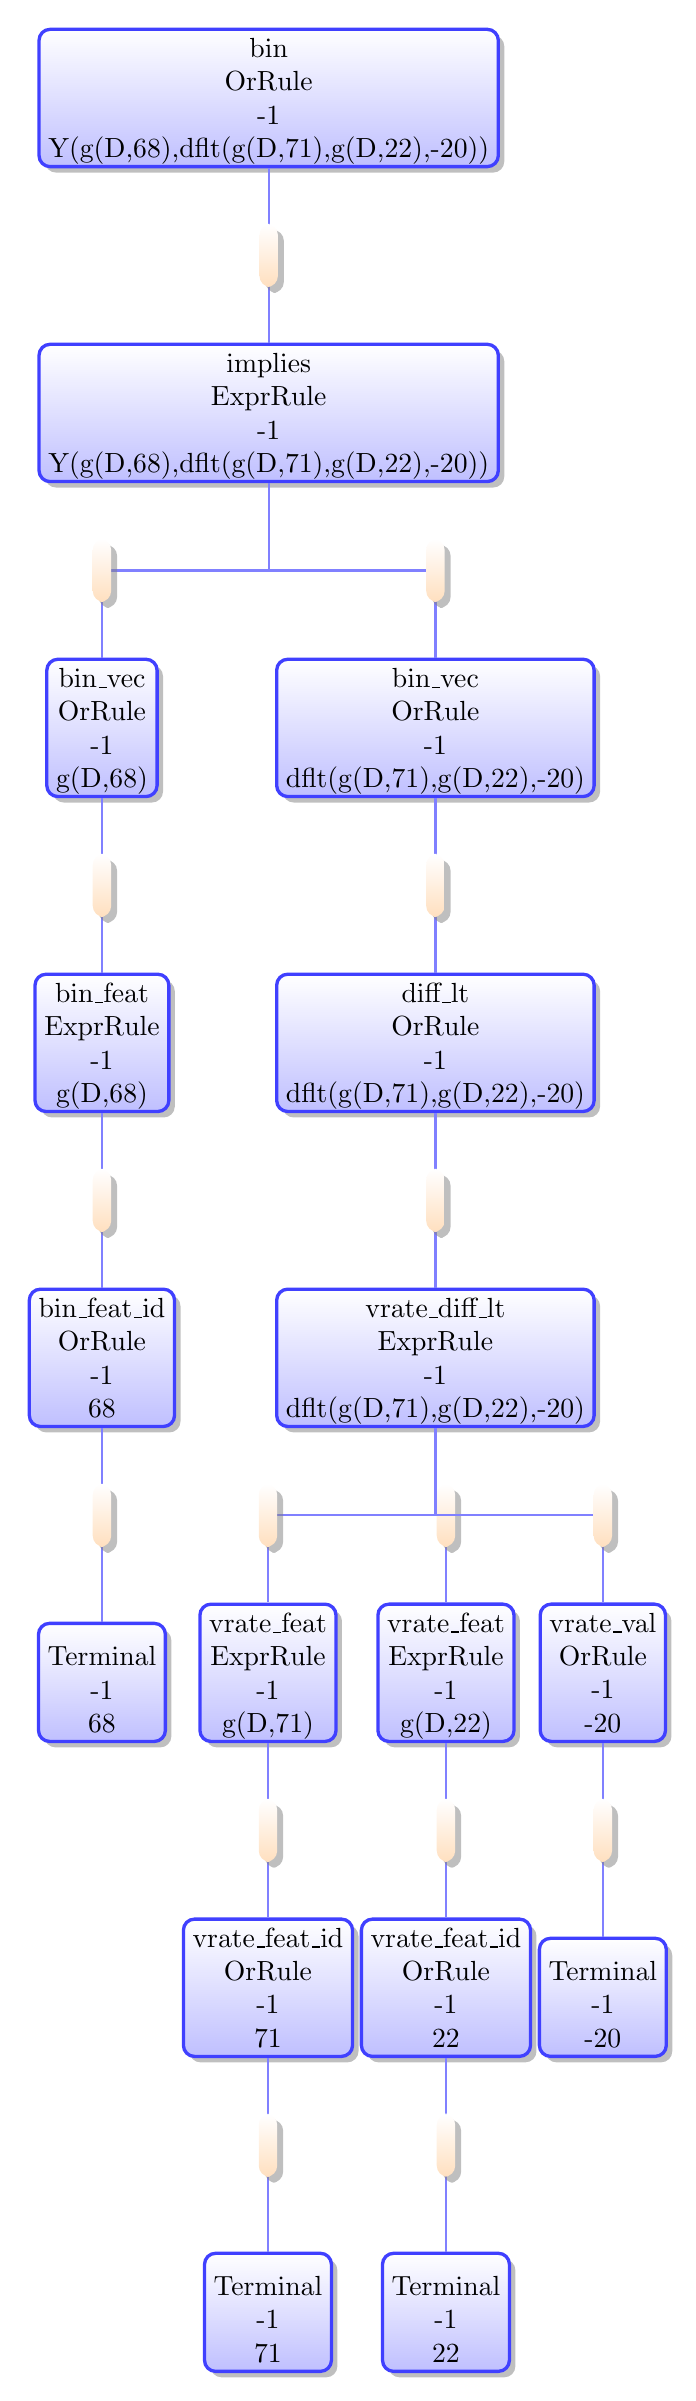
\begin{tikzpicture}[]
\Tree [.{bin\\OrRule\\-1\\Y(g(D,68),dflt(g(D,71),g(D,22),-20))}
\edge node[draw=none,bottom color=orange!25]{}; [.{implies\\ExprRule\\-1\\Y(g(D,68),dflt(g(D,71),g(D,22),-20))}
\edge node[draw=none,bottom color=orange!25]{}; [.{bin\_vec\\OrRule\\-1\\g(D,68)}
\edge node[draw=none,bottom color=orange!25]{}; [.{bin\_feat\\ExprRule\\-1\\g(D,68)}
\edge node[draw=none,bottom color=orange!25]{}; [.{bin\_feat\_id\\OrRule\\-1\\68}
\edge node[draw=none,bottom color=orange!25]{}; [.{\\Terminal\\-1\\68}
]]]]\edge node[draw=none,bottom color=orange!25]{}; [.{bin\_vec\\OrRule\\-1\\dflt(g(D,71),g(D,22),-20)}
\edge node[draw=none,bottom color=orange!25]{}; [.{diff\_lt\\OrRule\\-1\\dflt(g(D,71),g(D,22),-20)}
\edge node[draw=none,bottom color=orange!25]{}; [.{vrate\_diff\_lt\\ExprRule\\-1\\dflt(g(D,71),g(D,22),-20)}
\edge node[draw=none,bottom color=orange!25]{}; [.{vrate\_feat\\ExprRule\\-1\\g(D,71)}
\edge node[draw=none,bottom color=orange!25]{}; [.{vrate\_feat\_id\\OrRule\\-1\\71}
\edge node[draw=none,bottom color=orange!25]{}; [.{\\Terminal\\-1\\71}
]]]\edge node[draw=none,bottom color=orange!25]{}; [.{vrate\_feat\\ExprRule\\-1\\g(D,22)}
\edge node[draw=none,bottom color=orange!25]{}; [.{vrate\_feat\_id\\OrRule\\-1\\22}
\edge node[draw=none,bottom color=orange!25]{}; [.{\\Terminal\\-1\\22}
]]]\edge node[draw=none,bottom color=orange!25]{}; [.{vrate\_val\\OrRule\\-1\\-20}
\edge node[draw=none,bottom color=orange!25]{}; [.{\\Terminal\\-1\\-20}
]]]]]]];

\end{tikzpicture}
\end{document}
